\documentclass[conference]{IEEEtran}
\IEEEoverridecommandlockouts
% The preceding line is only needed to identify funding in the first footnote. If that is unneeded, please comment it out.
\usepackage{cite}
\usepackage{amsmath,amssymb,amsfonts}
\usepackage{algorithmic}
\usepackage{graphicx}
\usepackage{textcomp}
\usepackage{xcolor}
\def\BibTeX{{\rm B\kern-.05em{\sc i\kern-.025em b}\kern-.08em
    T\kern-.1667em\lower.7ex\hbox{E}\kern-.125emX}}

\begin{document}

\title{CENG 435 - Term Project - Part 1\\}

\author{
    \IEEEauthorblockN{1\textsuperscript{st} Hakan Sonmez}
    \IEEEauthorblockA{\textit{Department Engineering Computer Engineering} \\
    \textit{Middle East Technical University}\\
    Ankara, Turkey \\
    hakan.sonmez@ceng.metu.edu.tr}
    \and
    \IEEEauthorblockN{2\textsuperscript{st} Onur Tirtir}
    \IEEEauthorblockA{\textit{Department Engineering Computer Engineering} \\
    \textit{Middle East Technical University}\\
    Ankara, Turkey \\
    onur.tirtir@ceng.metu.edu.tr}
}

\maketitle

\begin{abstract}
\par The purpose of this work is to design and construct an unreliable network with end systems and intermediate nodes. The aim is to send messages on this network using Transmission Control Protocol (TCP) and User Datagram Protocol (UDP). We connect these different nodes containing different form of protocols with communication links. We then worked on conducting experiments on this network of multiple nodes measuring different delays.
\end{abstract}

\begin{IEEEkeywords}
server, client, socket, router, end-to-end delay, emulation delay, broker network topology, TCP, UDP, Acknowledgment
\end{IEEEkeywords}

\section{Introduction} \label{introduction}
\par In this work, we aimed to measure end-to-end delay with respect to different \textit{delay} configurations. We performed our work on a network consisting of five nodes, each of which has a different functionality. Along these nodes, we utilized different transport layer protocols to serve an end-to-end communication between \textit{source node} and \textit{destination node}. We also setup different delay configurations on the links between these nodes to perform our experiments. We will explain our network topology and configurations briefly in following Section \ref{design} briefly.

\par We will describe our implementation in different aspects in
Section \ref{implementation}. To explain, we will give details about how we establish the
connection between our nodes, protocols utilized from transport layer and run-time behavior performed by each node. We will also mention how we provided concurrency to our nodes for a better source utilization deeply.

\par As we mentioned above, we set different \textit{emulation delay} configurations in this work to measure end-to-end delay. We will describe and interpret results obtained from experiments in Section \ref{experimential} precisely. 

\par After giving a brief conclusion on overall work in Section \ref{conclusion}, we will finalize report. 

\section{Design} \label{design}
\par There are five nodes in the network due to the given topology: Source Node (s), Broker Node (b), Two Router Nodes (r1 and r2) and Destination Node (d). These nodes are connected to each other with \textit{communication links} as provided again in network topology. More specifically, Source node shares a link with Broker Node; Broker Node is connected to the routers and these routers are then finally connected to the Destination Node. The connection between Source node and Broker node is done using TCP, and all of the other connections are done using UDP. 
\par \textit{Source node} is only supposed to connect to Broker node and this connection is done by \textit{TCP}. This node is the one that is responsible of creating and sending this messages to the rest of the network. Hence we have decided that this node behaves like a \textit{client}. We have then discussed the terms packet,chunk and message. Source creates a message with a fixed size and this size is consistent throughout the topology. This size is the size of \textit{packets} throughout the network. We have also considered another approach where the message length to be dynamic, and send this length data first. However, as the topology and the scope of the project is fairly simple we have decided to use a fixed length. Message includes a body which is some arbitrary content. This message is sent to broker to be distributed on the whole network. We have considered and discussed about two different methods of starting the message creation and sending process. The first approach: After sending the data via TCP, this node then waits for an acknowledgment. This means that the Source node does not produce fast consecutive messages to send. Instead it sends a message, waits for an ACK then sends another message and so on. The second approach is that the Source node pumps messages and receives them simultaneously. This would imply that there is a multi-threaded design in the source. After discussing it we have decided to use the first method as it helps tracking the data across the network and helps measuring the delays needed. 

\par \textit{Broker node} is basically the main component of this network. It has three connections: one TCP connection to Source node and two UDP connections to both routers. Since there are multiple connections and the specification explains that there must be one script in each node; we have used a multi-threaded approach. This allows us to have multiple connection  operations made simultaneously in this node. The specification also states that the Broker Node has to start executing first. As a result, we have made the decision that all of the Broker parts of communication has to behave like a server. This also is consistent with the rest of the topology since the Source Node is a client and it basically needs to connect to a server via TCP. To explain briefly; Broker Node waits a message from Source, then sends it to one of the routers. After getting the message this node redirects and sends it to one of the routers. Similarly, Broker waits an ACK from router nodes, after getting the ACK, it transmits this acknowledgment to the link between Source node. 

\par \textit{Router Nodes'} purpose is to make the intermediate connection between Broker node and the Destination node. There is not a complicated task in these nodes. They either get the message from the Broker node and redirect it to the Destination node or get \textit{Acknowledgment} (ACK) from Destination node and transmit it to the Broker. Both of these connections are made with UDP. Since Router nodes connect to servers in both ends we have decided these nodes to behave like a client system.

\par \textit{Destination Node} is the node that the message finally reaches. Logically and due to the specifications, Destination node works like a server. So it has to always wait for a message. After receiving the message, it sends an Acknowledgment (ACK) message back to the link it received the message. The ACK includes basically a "Yes" or "No" message back to the Source node. This ACK message is sent via UDP to the router.

\section{Implementation} \label{implementation}
\par We set up five different scripts for five different nodes in our topology as described in Section \ref{design}. All of these scripts execute in the remote servers provided. As it is explained in the Section \ref{design} the data flow along the topology, we have two different partitions. First partition utilizes TCP in its underlying transport layer and second partition utilizes UDP. The TCP connections we have established are persistent. However, Since UDP is a \textit{connection-less} protocol a signal goes out automatically without determining whether the receiver is ready, or even whether a receiver exists.  First partition consists of \textit{source node} and \textit{broker node}. Second partition includes \textit{broker node}, two \textit{router nodes} and the \textit{destination node}. We have virtually put delays in the nodes with UDP connections to simulate a real life-like behavior. 

\par \textit{Source node} is the one generating the \textit{sensor data}. We generate a message of random \textit{sensor data}. This data includes a body containing the sensor reading. It is just a message in the form of a 32 byte randomly generated string. After sending this generated message, without it starts to wait for an \textit{Acknowledgment(ACK)} (for part 1) from network. The node just waits an ACK and does nothing else. Since we have to measure the time difference (\textit{end to end delay})between source node and destination node, we get and save the time-stamp of the exact time right after the source sends its data. Then, we also record the exact time right after the source node receives the related acknowledgment. This allows us to measure \textit{Round-Trip Delay Time}. \textit{End to end delay} is then the half of this value. We also have implemented a version where we have added a header to the message. The header included the time-stamp and we aimed to compare this time with the destination's time-stamp. However this failed as the local time between two nodes was pretty significant. Specifically in our case, we have observed that the local time of the Destination node was about 4 seconds behind. Hence this resulted in a meaningless negative delay. We have tried solving this problem with using \textit{Network Transfer Protocol (ntp)}. \textit{ntp} is a networking protocol for clock synchronization between computer systems over packet-switched, variable-latency data networks. We have tried fairly many attempts to synchronize both end systems.However, this synchronization task always resulted in a delay more than desired.
 
\par \textit{Broker node} does completely act as a server since the requirements state that it has to start executing first. It has three interfaces, one for connecting to \textit{source node} and the other two are for connecting to \textit{router nodes}. A \textit{TCP} socket is utilized via first interface to accept connection from \textit{source node} and two \textit{UDP} sockets are utilized on other two interfaces to communicate with routers. In order to implement this behavior we initiated three worker threads. These threads are to perform bidirectional communication between broker and routers and between \textit{source node}. Since the connection between source and broker is done via TCP, the corresponding socket we initiated has to be always open and connected. However, other two connections are done with using UDP. As a result there is not an ongoing connection between the routers. The broker does a send operation whenever and wherever the data comes. The thread responsible for receiving any form data (either message or ACK) does not send it via the socket it received. The data is basically transferred between threads via the sockets that are globally defined. While doing this data transfer between different threads with different connections there is no need to do any data processing since our implementation is an application layer one. Note that this data transfer allows the broker to handle both TCP and UDP. The ACK coming from one of the routers is sent to the source. Similarly the message coming from source node is sent to one of the routers. We have not used a routing table as the topology is quite simple and our aim in this part is not about improving \textit{throughput}, it is measuring delay. Distributing data is done by alternating between two routers. 

\par \textit{Router Nodes} do behave like a client since we have already established the other two connected nodes as servers. It would not make sense to connect two servers to each other both logically and network-wise. Both of these nodes behave exactly like each other with the minor difference being the related interfaces. There are two worker threads each in both of these router nodes. We have implemented a store and forward mechanism in the router nodes same as in the broker node. This mechanism ensures that the message to be send is always the predetermined message length. If the coming data is less than the message length the routers, or the broker node in this case, do not send the message immediately. Instead the node waits until the data has the sufficient length and then finally send it. This ensures that the message does not corrupt unless there is an error in the connection which we have no control over. 

\begin{center}
    \begin{figure*}[!hbtp]
        \centering
        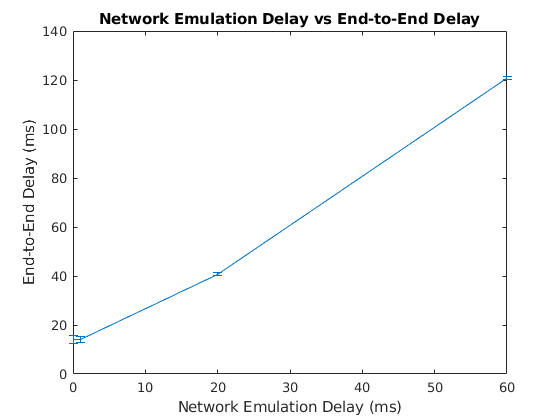
\includegraphics{plot.png}
        \caption{Network Emulation Delay vs End-to-End Delay}
        \label{delay}
    \end{figure*}
\end{center}


\par \textit{Destination Node} has two interfaces. They both use UDP connections between the Router Nodes. Since there are two connections this script also has two worker threads. Destination node behaves like a server due to the specifications. So, this node initially begins by trying to receive data from either of the routers with both of its threads. Note that since there is not a TCP connection between adjacent nodes, so if any of the routers send data while this node isn't waiting to receive, the data gets lost. After receiving the message, it produces an ACK. This ACK in our implementation is a one byte "True" or "False" value. This ACK then gets sent via the link its message came from. Even though it is not an issue in our implementation we have considered edge cases where there could be a race condition in any multi-threaded node. A node could be receiving and sending data in the same connection. It is not the case in our implementation since we do the data transfer sequentially. 

\section{Experimental Results} \label{experimential}

\par We performed our experiments for two (plus one) different link layer configurations -plus represents no tc/netem delay is applied-. These three configurations provide $1ms,\ 20ms\ and\ 60ms\ (\pm5ms)$ delays. When comparing our results, we thought that one packet will follow a path of $1$ edge with no additional delay and $2$ edge with \textit{tc} delay. 

\par We have sent $1000$ sensor-readings for each experiment and then took mean of delays for these $1000$ readings. We also have drawn error bars for each \textit{emulation delay/end to end delay pair}. To draw them, we focused on the confidence interval of $\% 95$ to generate delays with \textit{tc} and found $Z$ value to be $1.95$, then calculated these error bars.

\par In  Figure~\ref{delay}, we have four data points. $0$ -representing no tc delay- and $1ms\ (\pm5)ms$ can be hard to identify as they both have low error margins and they are represented nearly in graphic. To clarify, we have almost equal end-to-end delays for both cases, approximately $14ms$. We interpreted this result as $1ms\ \pm(5ms)$ delay does not have a huge effect on overall delay as the natural delay caused by the capacity of the links becomes more dominant. Moreover, error margin in no delay case is larger than the others. We interpreted this as behavior of links between hosts (with no additional delay) becomes more unpredictable as network's delay parameters(propagation delay, transmission delay, queueing delay etc) are the random variables as we discussed in class.

\par The other two data points represent $20ms\ (\pm5)ms$  and $50ms\ (\pm5)ms$ delays respectively. As we measured, we have nearly $40.8ms$ of delay for $20ms$ case and $120.7ms$ delay for $60ms$ delay case, which verifies our expectations from these experiments.

\par Looking the whole picture, as the \textit{tc} delay increases, it becomes more dominant as mentioned hence graphic becomes more linear.

\section{Conclusion}

\par We setup a topology with five nodes, each having a different job. The aim of this work was to observe the behavior of transport layer protocols, their effects on the end-to-end delay. We utilized \textit{tc/netem} to enrich our observations. The most time consuming part of this work for us was to \textit{debug} packets traveling between hosts in case of a bug. It was also dealing to research ways of measuring \textit{end-to-end} delay without utilizing \textit{RTT}. For the reasons mentioned in Section \ref{implementation}, we chose to measure first RTT and then to derive end-to-end delay from it.

\end{document}
